\subsection{Analytical Model}
	%Is it clear that we're trying to demonstrate a model that can be experimentally validated that has geothermal gradient? Is it also clear that we're hoping to conduct CBHE configuration optimization? Is it clear that we also hope to simulate seasonal performance of the CBHE? (The last one is very, very unclear. 
	We will be adapting the analytical model from Beier et al., which was developed to predict the thermal response from a CBHE with known geological parameters. This model was developed to adopt undisturbed ground temperature measurement from fiber optic temperature sensors (also referred to as distributed temperature sensor, or DTS). 
	
	%Explain the method, and the ADAPTION~ using a different reference temperature profile, also re-wrote the code into Python to be used as a class for different configurations to have its performance estimated and validated(use a plot to show its performance comparison?).
	Typically, the overall thermal resistance of a geothermal bore can be considered as the combined resistance of the bore and the ground. The bore thermal resistance can be affected by many parameters, including the pipe material, configuration of the heat exchanger as well as the thermal conductivity of the grout/backfill in the bore annulus. The ground resistance is dependent primarily on the thermal conductivity and the diffusivity of the surrounding formation. For a vertical BHE, its thermal resistance is the combined effect of pipe resistance and bore annulus grout resistance. As Kavanaugh and Rafferty pointed out, the terms of pipe and grout resistance can be combined into a single Equation~\ref{eq:Rb}. 
	
	\begin{equation}
		R_b = R_p + R_{grt} = R_{film} + R_{tube} + R_{grt} = 
		\frac{1}{\pi d_i h_{conv}} \frac{ln(d_o/d_i)}{2\pi k_p} + \frac{ln(d_b/d_o)}{2\pi k_{grt}}\label{Rb}
	\end{equation}
	
	This equation translates the thermal resistance of the pipe to the combination of the pipe resistances and the fluid film resistance inside the pipe wall. For coaxial borehole heat exchanger, this translates to both the film resistance at the inner pipe and the borehole wall, as well as the tube thermal resistance of both the outer and inner pipes. Calculation of the tube thermal resistance is relatively straight forward as the values required includes the diameter of the tubes and the thermal conductivity of it. However, as we are more interested in varying the configuration and insulation level at the borehole as we are showing conceptually in the section of the CBHE, we need to expand the existing definition of the shunt resistance of the borehole heat exchanger. Building on the existing expressions from Kavanaugh and Rafferty (2014) as well as Beier et al. (2012), we have a new expression of the shunt resistance of the borehole $R_{12}$. 

	%shunt resistance R12, refer to the borehole section plot. highlight geothermal gradient usage
	More specifically, the shunt resistance $R_p$, or sometimes referred to as $R_{12}$ of the CBHE is a parameter that we can modify to achieve different yield from a known location with certain geological condition. 
	%Our primary goal is to achieve an easy-to-use solution that compares the heat extraction capability of different R12, Rg and Rs.
	%Config
	From the schematic diagram, it is evident that any design intervention to change the performance of a CBHE needs to happen at the level that affect the shunt resistance. This expression allows us to evaluate the thermal resistances of CBHEs, we group the contributing variables into two categories: direct and indirect. Direct variables are the diameters of the inner and outer pipes, thermal conductivity of the pipe material, and the thickness and material of the insulation material inside the inner pipe. The flow rate entering the CBHE is the indirect variable, which not only affect the convective heat transfer coefficients contributing to the film thermal resistances. To provide a more accurate description of the thermal resistance of the shunt resistance, expression of $R_{12}$ needs to be updated as Equation~\ref{eq:R12}. This includes the film thermal resistances at the heat exchanger surfaces, and the thermal resistances that represents the conductive heat transfer through the pipe and insulation materials, i.e. $R_{pw1}, R_{ins}, R_{pw2}$. More explicitply, these individual expressions can be written as Equation~\ref{eq:RR12}, where the overall shunt resistance may change with respect to different CBHE configurations. This is also expressed in Figure~\ref{fg:cbhesec}. 
	    
	    \begin{equation}
          R_{12} = R_{fi} + R_{pw1}+ R_{ins}+ R_{pw2} + R_{fo} \label{eq:R12}
        \end{equation}
        
        \begin{equation}
            Nu = \frac{hL}{k}\label{eq:Nuhx}    
        \end{equation}
        \begin{equation}
              \left\{
              \begin{aligned}
              & R_{fi} = \frac{1}{\pi d_{pi} h_{pi}}\\
              & R_{pw1} = \frac{ln(\frac{d_{pw1}}{d_{pi}})}{2\pi k_{pw}}\\
              & R_{ins} = \frac{ln(\frac{d_{pw2}}{d_{pw1}})}{2\pi k_{ins}}\\
              & R_{pw2} = \frac{ln(\frac{d_{po}}{d_{pw2}})}{2\pi k_{pw}}\\
              & R_{fo} = \frac{1}{\pi d_{po} h_{po}}
              \end{aligned}
              \right. \label{eq:RR12}
        \end{equation}
		
		\begin{figure*}[h!]
			\centering
			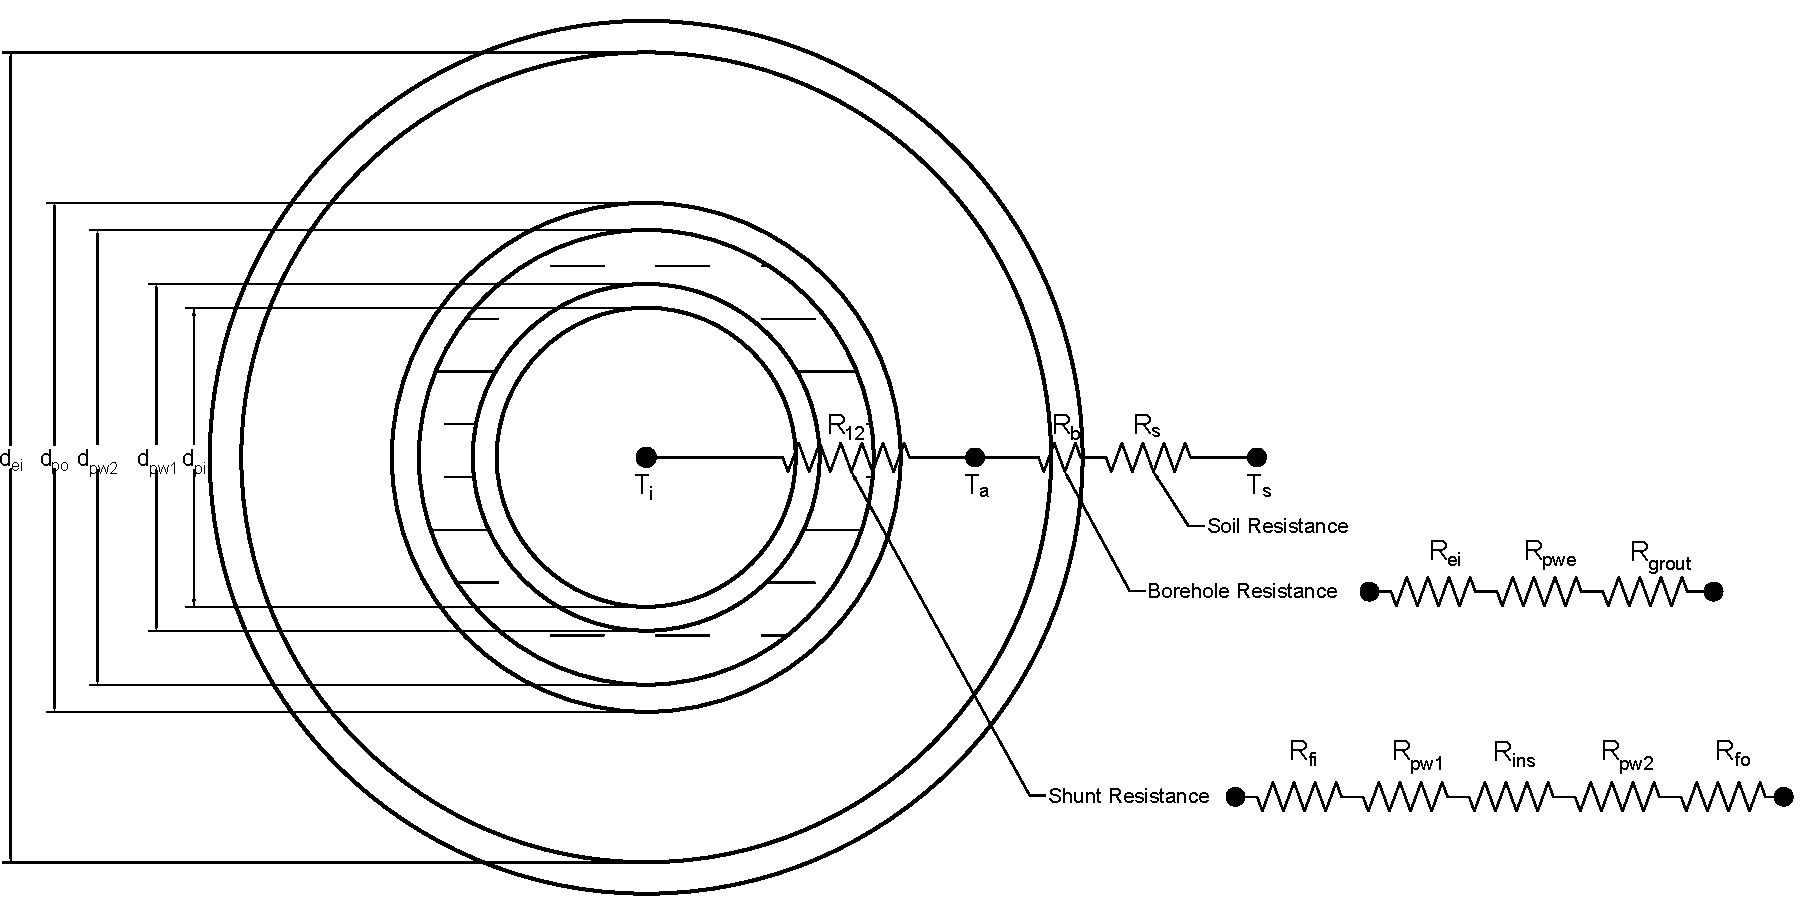
\includegraphics[width=0.8\textwidth]{data/CBHE_CrossSection}
			\caption{Schematic diagram of thermal resistance calculation for borehole.}\label{fg:cbhesec}
		\end{figure*}
	%These are the parameters that we are primarily interested in varying when changing the R12
	
If we may overtly simplify the entangled the relationship between the depth, performance and cost can be generalised into a statement: the further down the reach of the borehole, the higher the bottom of borehole temperature, and the larger the drilling costs and operational (pumping costs). And to improve the heat exchanger capability of any CBHE, we will therefore need to either change the configuration of the CBHE, or the location of the CBHE. This can be categorized into either shunt-resistance-related parameters and the site-specific parameters. 


%How the model works? 

	\subsubsection{Diameter, insulation level, and flow rates}
	Diameters, insulation level and flow rates are parameters that we may subjectively alter to modify the performance of borehole heat exchangers. 
	%insulation
	To better utilise the geothermal energy that is returned to the ground surface, insulating the inner pipe of CBHEs so that the heat transfer between the inner tube and annulus will not short-circuit the heat extraction in the CBHE.  
	The resulting importance of adding insulation on the inner pipe was highlighted in a few previous publications \cite{li_synthesis_2014,guillaume_analysis_2011}but was found to be not economically feasible for project proposal\cite{dijkshoorn_measurements_2013}. 
	One such study came from Dijkshoorn et al. , in which the construction and measurement of a 2500m deep well helped to validate the modelling of satisfying borehole performance over 30 years when using the borehole output to drive a climate control adsorption chiller. However, their results did not support the extra investment of adding an insulated inner pipe for the borehole - the entire project came to a halt at such.
	Additionally, despite acknowledging the possibility of added thermal benefit by inserting an insulated inner pipe, this was not further pursued due to cost constraints. In a very recent publication, the effect of changing the pipe configuration to achieve better thermal performances, but does not vary the design and environmental (specifically on the geothermal gradient) parameters component-by-component in CBHE design\cite{liu_numerical_2019}.

	
	%Depth
	\subsubsection{Geothermal gradient and thermal conductivity}
	Using the same set of method outlined by Beier et al. \cite{beier_situ_2012}, it is possible to use an arbitrary temperature profile as the the undisturbed ground temperature and solve for corresponding ground temperature. 
	
	Another modification of the method we're adapting is described as Equation~\ref{eq:bcggradient}, where the temperature distribution along the depth of CBHE can be considered constant at locations that are infinitely far away from the center of the test well.  
	
	\begin{equation}
            \frac{\partial T_{DS}}{\partial z_D}(r_D\rightarrow \infty, t_D,z_D) = g_D(z_D) \quad t_D > 0\label{eq:bcggradient}
    \end{equation}
	
	Geothermal gradient, thermal conductivity, are parameters that varies objectively, but varies significantly enough spatially that could also affect the performance of a CBHE. Addressing the presence of geothermal gradient is therefore extremely important when the proposed boreholes are deeper rather than shallower. Existing studies show that geothermal gradient may vary between 1 to 5 Kelvin per hundred meters' depth\cite{holmberg_thermal_2016,shrestha_assessment_2018}.

	%Validation of the analytical model
	
	%Comparison with the constant ground temperature solution
		
	%Thermal resistances. Look at the GTRI report also for a good reference.
\subsection{Analytical Solution}
	For each time step, a new analytical solution can be solved along different t, r and depth in CBHE. Following the same set of method 
	

	
	%Python
	As we are interested in the possible benefits of designing CBHEs better through different combinations of configurations, we are primarily interested in creating a lightweight algorithm that allows us to compare the expected thermal response outcomes (particularly the thermal resistances or heat extracted) between the different configurations. We therefore adapted the analytical method from Beier et al. \cite{beier_borehole_2013} with the following modifications: expanded the shunt resistance expression to allow for extra thermal insulation inside the inner pipe; adopted geothermal gradient into the undisturbed ground temperature during the solving of the target temperature function and translated the original analytical model from MathCAD into Python as a class that allows parallel comparison of the resulting thermal resistance of the boreholes.

	Therefore, for every time step during a simulated hypothetical time step, the corresponding analytical solution can be calculated for a given radius, depth and time since operation. Using Laplace transformation, the heat exchange within the central and annular flow can be solved using the Navier-Stokes equation with boundary and initial conditions. As all the variables were converted into dimensionless form, including the time component, the analytical solution requires an inverse Laplace transform to calculate temperatures in the time domain. The detailed solution of the energy equations using the initial and boundary conditions can be found in the appendix for the annulus as inlet scenario. We used the Stehfast algorithm following Beier's example in his 2013 paper\cite{beier2013} to perform the inverse laplace transformation. 

\subsection{Validation of adapted model}
	To confirm the validity of our adapted model, we want to compare the temperature profile that we can create by modeling the temperature distribution inside the CBHE. The parameter we used as the model input are as the followings shown in Table~\ref{tb:inputs_val}. 
	
	\begin{table}[h!]
            \begin{center}
            % \small\addtolength{\tabcolsep=0.11cm}{-5pt}
            % \scalbox{0.7}{
            \tabcolsep=0.11cm
%            {\singlespacing}
            \begin{tabular}{lcl}
                \hline
                Parameter & Symbol & Value\\
                \hline
                Borehole radius & $r_{b}$ & 115 mm\\
                Active heat exchanger length & L & 170 m\\
                Inner pipe outer radius & $r_{po}$ & 40 mm\\
%                Inner pipe wall thickness & $r_{po}$-$r_{pi}$ & 2.4 mm\\
                External pipe outer radius & $r_{eo}$ & 114 mm\\
                Inner pipe thickness & $d_{pp}$ & 2.4 mm\\
                External pipe thickness & $d_{ep}$ & 0.4 mm\\
                Inner and external pipe wall thermal conductivity & $k_{pp}$,$k_{ep}$ & 0.40 W/(K$\cdot$m)\\
                Ground thermal conductivity & $k_{s}$ & 3.15 W/(K$\cdot$m)\\
                Ground volumetric heat capacity & $c_{s}$ & 2.24 $\times$ $10^6$ J/(K$\cdot$$m^3$)\\
                Water flow rate & w & 0.58 $\times 10^{-3}m^3/s$\\
                Water density (at 15$^{\circ}$C) & $\rho$ & 999 kg/$m^3$\\
                Water volumetric heat capacity (at 15$^{\circ}$C) & $c_{w}$ & 4.19 $\times$ $10^6$ J/(K$\cdot$$m^3$)\\
                Water thermal conductivity (at 15$^{\circ}$C) & $k_{w}$ & 0.59 W/(K$\cdot$m)\\
                Water dynamic viscosity (at 15$^{\circ}$C) & $\mu_{w}$ & 1.138 $\times$ $10^{-3}$ kg/(m$\cdot$s)\\
%                Water Prandtl number & Pr & 8.09 \\
%                Heat input rate & Q & 6360 $W$\\
                Reference soil surface temperature & $T_{rs}$ & 8.9$^\circ$C\\
                % Average ground temperature & $T_{s}$ & 8.4$^\circ$C\\
                Nondimensional temperature of soil & $T_{DS}$ &\\
                Nondimensional temperature of inlet/outlet & $T_{D1},T_{D2}$ &\\
                \hline
            \end{tabular}
            \end{center}
            \caption{\label{table 2}Nomenclature, input parameters used in determining the performance of CBHE.}\label{tb:inputs_val}
	\end{table} 
	
